\chapter{Vibe Coding} 

Vibe coding is one of the most successful and widely appreciated applications of LLM and agentic AI. Many LLM service providers such as OpenAI and Anthropic provide vibe coding services for their subscribers. In this chapter, vibe coding is introduced with Anthropic Claude Code used as an example.

Notice that vibe coding is continuously evolving. The materials introduced in this notebook only reflect the development up to the writing.

\section{Different Ways of Coding}

In the past few years, LLM and agentic AI have revolutionized the way developers code. Up till this writing, there have been at least the following different ways of coding, and it is continuously evolving.
\begin{itemize}
  \item Conventional coding
  
  A developer codes in a conventional \myabb{Integrated Development Environment}{IDE} which is little more than just a text editor. All codes are inserted into the scripts manually. The IDE is often able to detect syntax error and compile the code.
  
  Example: VS Code without AI-featured extensions.
  
  \item Coding with autocompletion
  
  The AI predicts the intention of the developer by looking at the existing codes and comments, and automatically fill in the next few lines of codes. The developer can modify the filled contents when necessary.
  
  Autocompletion is effective when the contents to be filled is simple, self-contained, and pattern-wise consistent with existing codes, but may struggle with fully automatically generating a long portion of codes for complex functions.
  
  Example: VS Code with GitHub copilot extension.
  
  \item Agentic programming
  
  The IDE is incorporated with a chatbox. The developer can put their comprehensive requests into the chatbox, and the AI is able to review, modify or generate files in the project directory to achieve the goal. When the AI agents modify the codes, the developer can review the modification in real-time. The reviewer can accept or reject each changes before testing the program. The developer can raise new requests during the development by interacting with the AI using the chatbox. Should their be any error message, the AI is able to view the message and revise the code accordingly. 
  
  Compared with autocompletion, in agentic programming the AI agents are allowed to read and write files in the project folder, and iteratively and recursively program and test the codes. It leverages the level of automation in coding and requires much less human involvement. However, the AI agents can only reach everything in the project folder and have no means to access any resources in the outside world, for example, to query the Internet for the latest libraries or to automatically raise a pull request on GitHub when a feature is developed.
  
  Example: VS Code with GitHub copilot extension in ``Agent'' mode.
  
  \item Vibe coding
  
  In vibe coding, there is not necessarily an IDE. The developer puts the requirements in markdown files prior to the programming, and start the AI from the \myabb{Command Line Interface}{CLI}. The AI reads the requirements, plans the developing procedures, performs and tests the programming iteratively. Different from agentic programming, the AI is able to equip MCP tools, skills and plugins to better coordinate the development of the project. For example, it can query the Internet for latest user manuals for the libraries, manage the project in Jira, update the project in GitHub, and so on. The developer is able to interact with the AI in CLI using natural language. They can supervise the coding process should they wish to. They can also leave everything to the AI, including the programming, testing, debugging and documentation.
  
  In both agentic programming and vibe coding, the programming can be done by multiple AI agents. In vibe coding, more complicated frameworks are supported, and the AI chooses the framework. Hence, vibe coding is often considered more automated than agentic programming. With vibe coding, it is possible to let the machine run by itself for a few days with no human interactions to deliver a project. However, the amount of token consumption of vibe coding is often considerably larger than agentic programming. The quality of the job largely depends on the precision of the instruction files and tools. It is challenging for the developer to work collaboratively with the AI to code or debug due to the massive amount of codes automatically generated by the AI.
  
  Example: Anthropic Claude Code, OpenAI Codex, AMP, VS Code with GitHub copilot extension in ``Plan'' mode.
  
\end{itemize}

In the context of vibe coding, the developer does not need to program a single line of code. Instead, they need to construct the requirement documents and equip the AI with necessary tools. They are known as the \mync{context engineer}, an expansion of prompt engineer role.

\subsection{Project Tree}

The project tree of a vibe coding environment may look like Fig. \ref{fig:claude_vibe_tree}. Notice that Claude Code is used as an example. Other vibe coding tools such as Codex may have a slightly different project tree structure.

\begin{figure}[!htb]
	\centering
	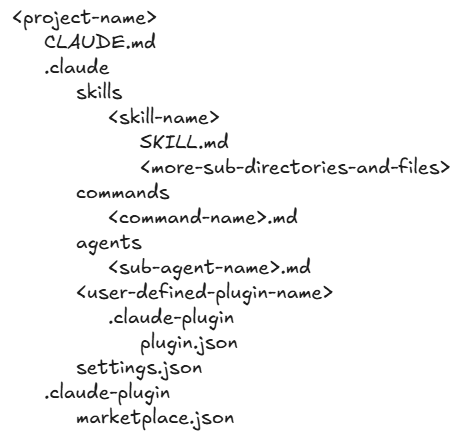
\includegraphics[width=0.6\textwidth]{./chapters/part-4/figures/claude_vibe_tree.png}
	\caption{An example of the project tree of a Claude Code vibe coding project.}
	\label{fig:claude_vibe_tree}
\end{figure}

In the project tree, \verb|CLAUDE.md| is compulsory as it serves as the instruction to the AI on what to do with the project. The rest files and subdirectories such as the \verb|.claude/skills| are optional and they are used to expand the capability of the AI. More about them will be introduced in the coming sections.

\subsection{Pros and Cons}

While vibe coding is indeed very powerful as will be illustrated by the examples in the coming sections, it has restrictions. The advantages and disadvantages of vibe coding over conventional coding are discussed in this section.

\section{Code with Vibe Coding}

This section introduces vibe coding with Claude Code. Many concepts and techniques introduced in this section can be transferred to other vibe coding tools such as OpenAI Codex and AMP.

\subsection{Installation}

\subsection{Project Initialization}

\subsection{Tools, Skills and Plugins}

\subsection{Sub Agent}

\section{Example: D\&D Co-player Project}
